Using the unfolding procedure outlined in Section~\ref{sec:unfolding}, we can unfold the reconstructed level $\Sigma E_{T}$ distribution for inclusive jet and dijet events.
Figure~\ref{fig:unfolded_pt} shows the unfolded level average $\Sigma E_{T}$ as a function of leading jet $p_{T}$ for inclusive jet (left) and dijet (right) events with a selection of systematic variations.
\begin{figure}
    \centering
    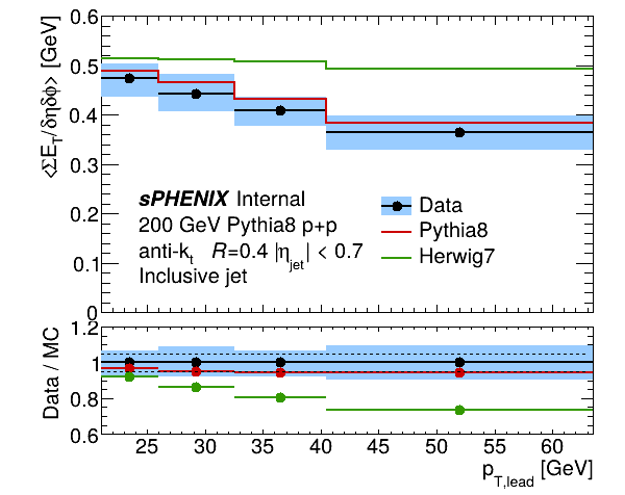
\includegraphics[width=0.48\linewidth]{Figures/h_result_inclusive.png}
    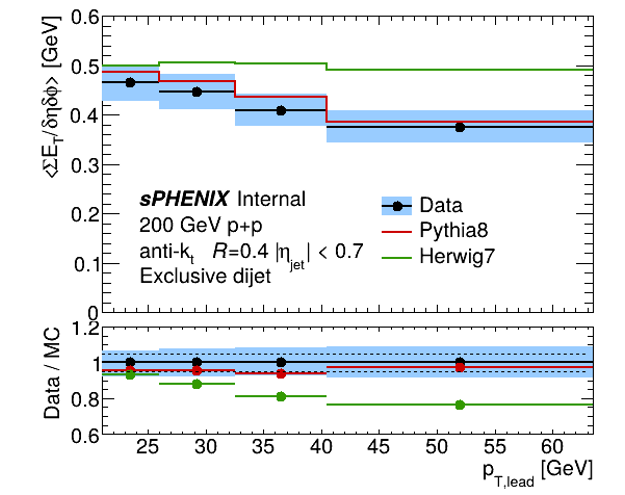
\includegraphics[width=0.48\linewidth]{Figures/h_result_dijet.png}
    \caption{Unfolded level average $\Sigma E_{T}$ as a function of leading jet $p_{T}$ for inclusive jet (left) and dijet (right) events with comparison to Pythia8.}
    \label{fig:unfolded_pt}
\end{figure}

Similar trends are seen between the two event selections, with the average $\Sigma E_{T}$ decreasing with leading jet $p_{T}$ and slightly lower than the truth result from Pythia8.
While the systematic uncertainty on the measurements are large, the uncertainties are highly correlated between different leading jet $p_{T}$ bins and thus the trend of the measurement is more robust than the overall normalization.
The overall scale uncertainty is dominated by the hadronic response uncertainty and can be factored out when making comparisons between different jet $p_{T}$ bins or different event selections.
Plots comparing the results of the inclusive jet and dijet selections will be included in the final note to more clearly show the strong agreement. 